% ============================================================
%  CHAPITRE 2 : ANALYSE ET CONCEPTION
% ============================================================

\cleardoublepage
\thispagestyle{empty}

\titleformat{\chapter}[display]
  {\normalfont\bfseries\color{black}\centering}
  {\Large CHAPITRE \thechapter}
  {20pt}
  {\Huge}[\clearpage]
\titlespacing*{\chapter}{0pt}{150pt}{0pt}

\chapter{Analyse et Conception}
\label{ch:analyse_conception}

\titleformat{\chapter}[display]
  {\normalfont\bfseries\color{black}\centering}
  {\Large CHAPITRE \thechapter}
  {20pt}
  {\Huge}
\titlespacing*{\chapter}{0pt}{80pt}{40pt}

% ============================================================
\section{Introduction}
% ============================================================

Apres avoir pose le contexte du projet et specifie les besoins dans le
chapitre precedent, ce deuxieme chapitre aborde la phase d'analyse et de
conception. C'est une etape charniere : elle transforme des besoins exprimes
en langage naturel en une architecture logicielle precise et documentee,
sur laquelle le developpement pourra s'appuyer directement.

Nous presentons ici les outils et methodes de modelisation retenus, les
acteurs du systeme et leurs interactions a travers les diagrammes de cas
d'utilisation, les diagrammes de sequence illustrant les scenarios
principaux, ainsi que le diagramme de classes qui constitue la base
structurelle de la base de donnees de l'application.

% ============================================================
\section{Methodes et outils de modelisation}
% ============================================================

\subsection{Langage de modelisation UML}

UML (Unified Modeling Language) est un langage de modelisation graphique
standardise, largement adopte dans le domaine du genie logiciel. Il permet
de visualiser, specifier et documenter les differentes dimensions d'un
systeme, aussi bien sa structure statique que son comportement dynamique.

Dans le cadre de ce projet, UML a ete utilise pour produire trois types
de diagrammes complementaires :

\begin{itemize}
  \item Les \textbf{diagrammes de cas d'utilisation}, qui decrivent les
        interactions entre les acteurs et le systeme, et permettent de
        valider que l'ensemble des besoins fonctionnels est bien couvert.
  \item Les \textbf{diagrammes de sequence}, qui retracent le deroulement
        chronologique des echanges entre les composants du systeme lors
        des scenarios les plus importants.
  \item Le \textbf{diagramme de classes}, qui represente la structure des
        donnees, les entites du domaine et leurs relations, et sert de
        reference directe pour la conception de la base de donnees.
\end{itemize}

\subsection{Identification des acteurs}

Un acteur est toute entite externe qui interagit avec le systeme. Pour
l'application WAVE, quatre acteurs principaux ont ete identifies.

\textbf{L'Admin} est l'administrateur de la plateforme. Il dispose des
acces les plus etendus : il peut gerer les comptes managers, le catalogue
de produits, et definir les objectifs mensuels de chaque manager. Il herite
egalement de toutes les fonctionnalites du manager.

\textbf{Le Manager} est le commercial de l'agence. Il prend en charge le
suivi quotidien des clients : gestion des paiements, attribution des
licences, suivi des contrats et des relances, pilotage du pipeline
commercial et consultation des tickets de support.

\textbf{Le Client} est l'utilisateur final de l'espace client. Il
consulte ses licences actives, ses factures et ses contrats, soumet des
tickets de support et peut passer des commandes directement en ligne via
PayPal.

\textbf{Le Scheduler (Cron)} est un acteur systeme qui represente le
planificateur de taches de Laravel. Il declenche automatiquement des
traitements en arriere-plan : verification quotidienne des licences,
envoi d'emails de rappel et generation du rapport mensuel.

% ============================================================
\section{Diagrammes de cas d'utilisation}
% ============================================================

Les diagrammes de cas d'utilisation ont ete organises par acteur afin
de garder une lecture claire malgre le nombre important de fonctionnalites
couverts par la plateforme. Trois diagrammes ont ete produits, chacun
couvrant un perimetre fonctionnel distinct.

\subsection{Diagramme de cas d'utilisation -- Scheduler, Gestion Clients
            et Gestion Factures}

Le premier diagramme (Figure \ref{fig:dcu1}) regroupe les fonctionnalites
liees a la gestion des clients, a la facturation et aux automatisations
declenchees par le planificateur de taches.

Cote gestion des clients, le manager peut lister, rechercher, creer,
modifier et supprimer des fiches clients. Il peut egalement provisionner
un compte utilisateur pour un client et exporter la liste au format CSV.
La consultation de la fiche client sert de point d'entree pour acceder
aux autres modules : paiements, licences, contrats et relances.

Cote facturation, le manager cree des factures avec numerotation
automatique au format \texttt{FAC-YYYY-NNNN}, les modifie, les supprime
et peut telecharger chaque facture en PDF.

Le Scheduler prend en charge trois automatisations : il verifie et met
a jour le statut des licences chaque jour, envoie des rappels d'expiration
sept jours avant l'echeance, envoie des rappels de retard de paiement
chaque lundi, et genere un rapport mensuel envoye automatiquement aux admins.

\begin{figure}[H]
  \centering
  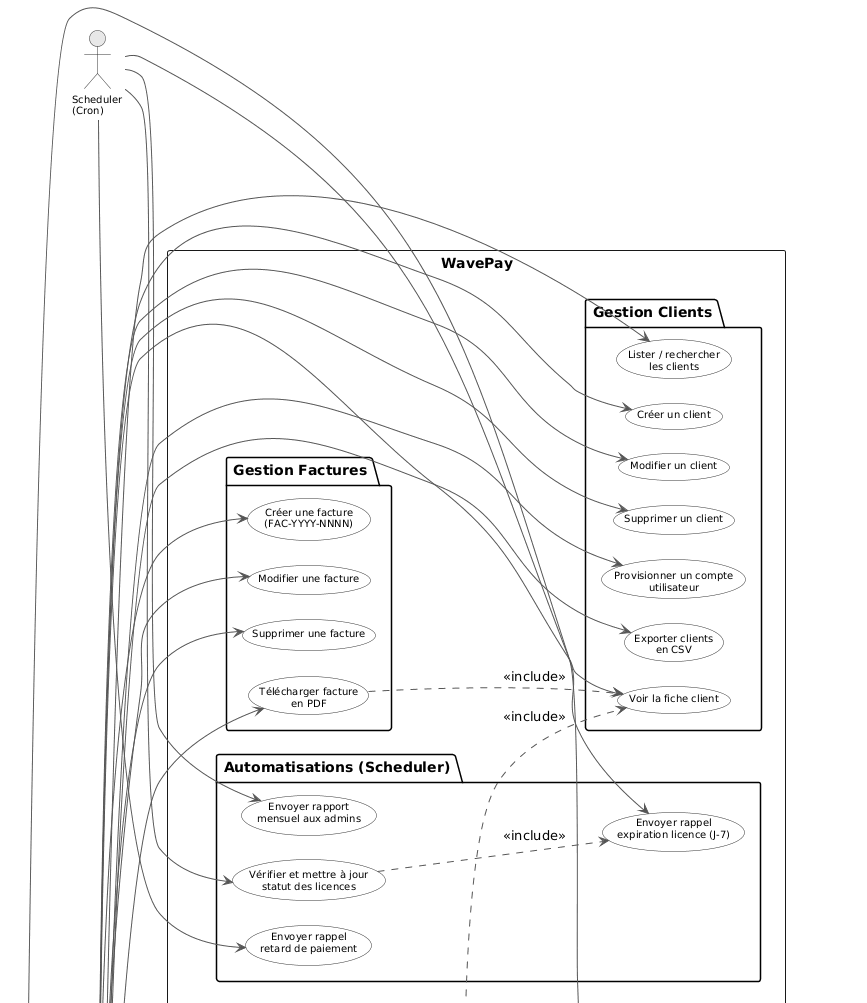
\includegraphics[width=0.82\textwidth]{diagrammes-casdutilisations/Diag-Cas-Utilisation-1.png}
  \caption{Diagramme de cas d'utilisation -- Scheduler, Clients et Factures}
  \label{fig:dcu1}
\end{figure}

\subsection{Diagramme de cas d'utilisation -- Manager}

Le deuxieme diagramme (Figure \ref{fig:dcu2}) est entierement dedie
au role Manager et couvre l'ensemble de son perimetre operationnel.

La \textbf{gestion des contrats} permet de creer, modifier et supprimer
des contrats, et de visualiser directement depuis le tableau de bord
les contrats qui expirent bientot.

Le module de \textbf{relances commerciales} (follow-ups) offre la
possibilite de creer, modifier et supprimer des relances associees a
un client, et de les marquer comme effectuees une fois realisees.

Le \textbf{pipeline commercial} centralise la gestion des opportunites
CRM : lister, creer, modifier et supprimer des opportunites avec leur
montant estime et leur date de cloture prevue.

La section \textbf{dashboard et reporting} donne acces au tableau de
bord avec KPIs et graphique des revenus mensuels, ainsi qu'au journal
d'activite (audit log Spatie) par client.

Enfin, la \textbf{gestion des paiements} couvre l'enregistrement, la
modification, la suppression et l'export en PDF du releve de paiements,
tandis que la \textbf{gestion des licences} permet d'attribuer, de
revoquer et de consulter les licences d'un client.

\begin{figure}[H]
  \centering
  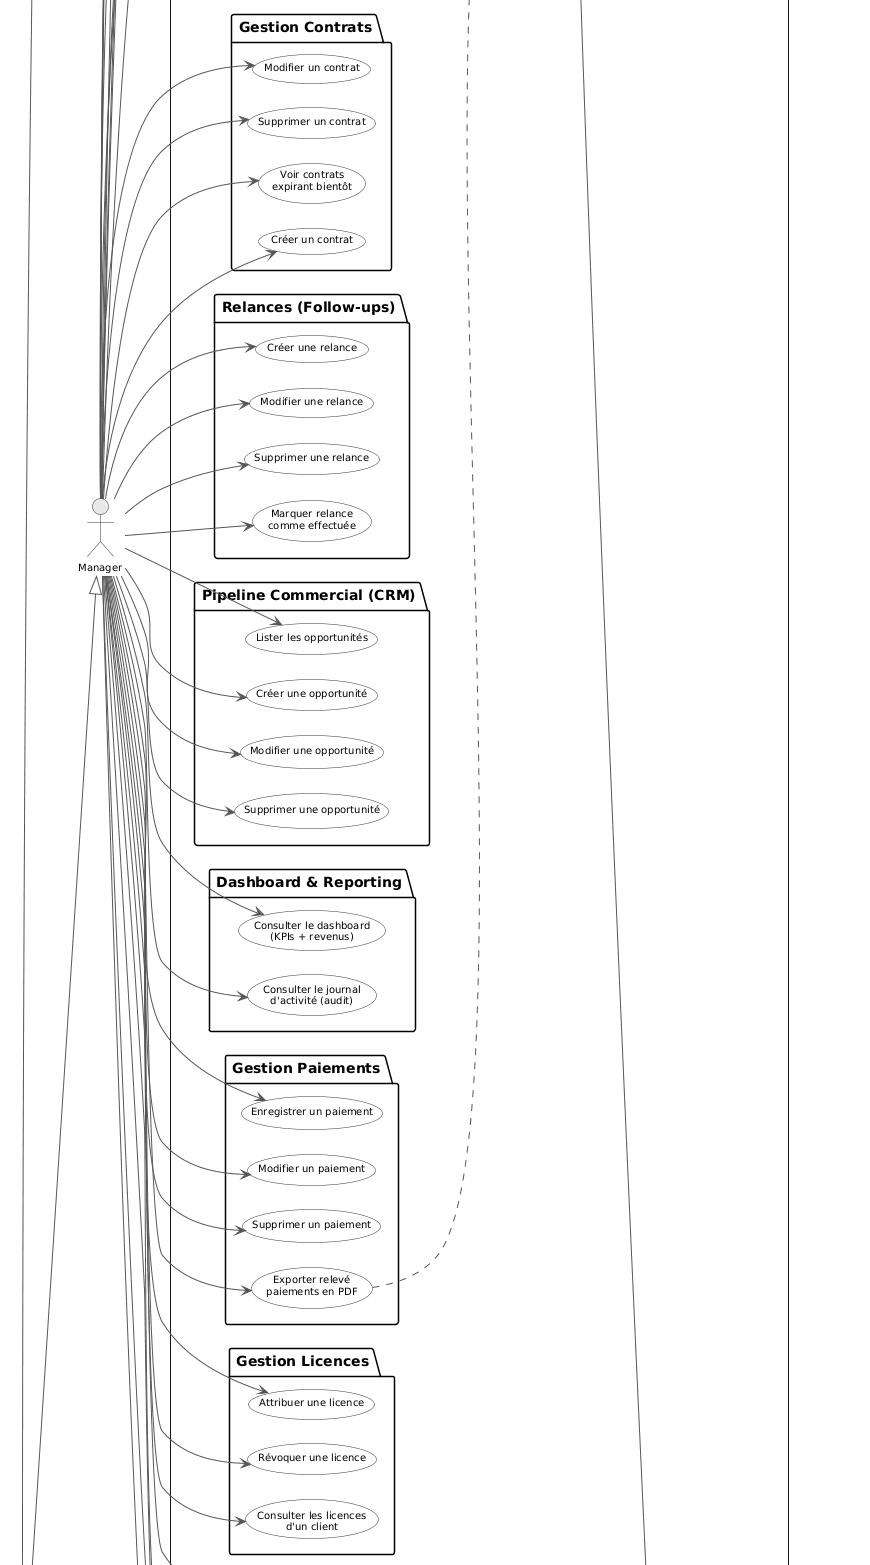
\includegraphics[width=0.72\textwidth]{diagrammes-casdutilisations/Diag-Cas-Utilisation-2.png}
  \caption{Diagramme de cas d'utilisation -- Manager}
  \label{fig:dcu2}
\end{figure}

\subsection{Diagramme de cas d'utilisation -- Admin et Client}

Le troisieme diagramme (Figure \ref{fig:dcu3}) regroupe les cas
d'utilisation specifiques a l'Admin et au Client.

Du cote \textbf{Admin}, le module d'authentification est commun a tous
les roles (connexion, deconnexion, consultation du profil via
\texttt{/me}). Le module de gestion admin lui permet de gerer les
managers en CRUD complet, de gerer le catalogue produits, d'activer
ou desactiver un produit et de definir les objectifs mensuels de chaque
manager. Il partage egalement l'acces aux tickets de support en vue
manager.

Du cote \textbf{Client}, l'espace personnel lui donne acces a son profil
et a ses licences actives, a ses factures avec telechargement PDF, a ses
contrats et a ses notifications in-app avec possibilite de les marquer
comme lues. Il peut exporter son releve personnel en PDF. Le module
boutique lui permet de parcourir le catalogue de produits actifs et de
passer une commande, ce qui inclut la redirection vers PayPal et la
confirmation du paiement via l'API PayPal SDK.

\begin{figure}[H]
  \centering
  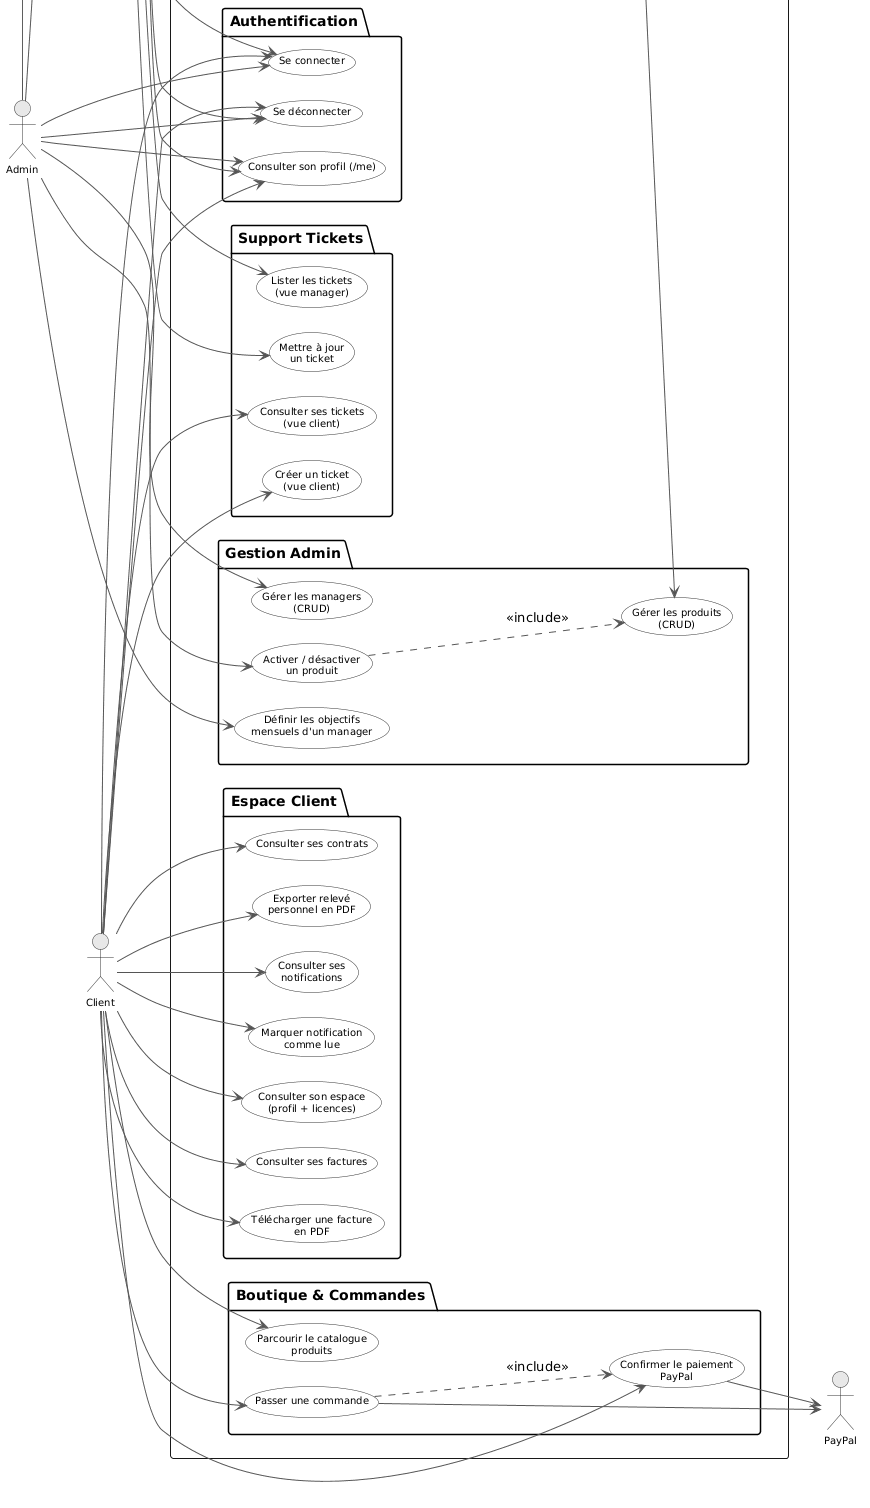
\includegraphics[width=0.82\textwidth]{diagrammes-casdutilisations/Diag-Cas-Utilisation-3.png}
  \caption{Diagramme de cas d'utilisation -- Admin et Client}
  \label{fig:dcu3}
\end{figure}

% ============================================================
\section{Diagrammes de sequence}
% ============================================================

Les diagrammes de sequence permettent de representer dans l'ordre
chronologique les echanges entre les differents composants du systeme
pour un scenario donne. Trois scenarios ont ete selectionnes parmi les
plus representatifs et les plus complexes de l'application.

\subsection{Sequence 1 -- Authentification et redirection par role}

Ce premier diagramme de sequence (Figure \ref{fig:seq1}) couvre deux
scenarios etroitement lies : la connexion d'un utilisateur et l'acces
a une route protegee.

Lors de la connexion, l'utilisateur saisit son email et son mot de passe
dans le formulaire React. Le frontend envoie une requete POST vers
\texttt{/api/v1/login}. Le backend interroge la base de donnees pour
verifier l'existence du compte et la validite du mot de passe. En cas
d'echec, une reponse 401 est retournee avec un message d'erreur affiche
cote client. Si les identifiants sont corrects, un token Sanctum est genere
et stocke dans la table \texttt{personal\_access\_tokens}. Le backend
retourne ce token accompagne des informations de l'utilisateur (id, nom,
role). Le frontend stocke le token dans le \texttt{localStorage} sous
la cle \texttt{wave\_token}, puis redirige automatiquement selon le
role : vers \texttt{/admin/dashboard} pour un admin, vers
\texttt{/manager/dashboard} pour un manager, ou vers \texttt{/client}
pour un client.

Lorsque l'utilisateur navigue vers une route protegee, le frontend joint
automatiquement le token dans l'en-tete HTTP \texttt{Authorization: Bearer}.
Le middleware Sanctum verifie la validite du token dans la table
\texttt{personal\_access\_tokens}. Si le token est invalide ou expire,
le backend retourne un 401, l'intercepteur Axios purge le \texttt{localStorage}
et redirige vers la page de connexion. Si le token est valide, l'utilisateur
est injecte dans la requete et l'acces est accorde.

\begin{figure}[H]
  \centering
  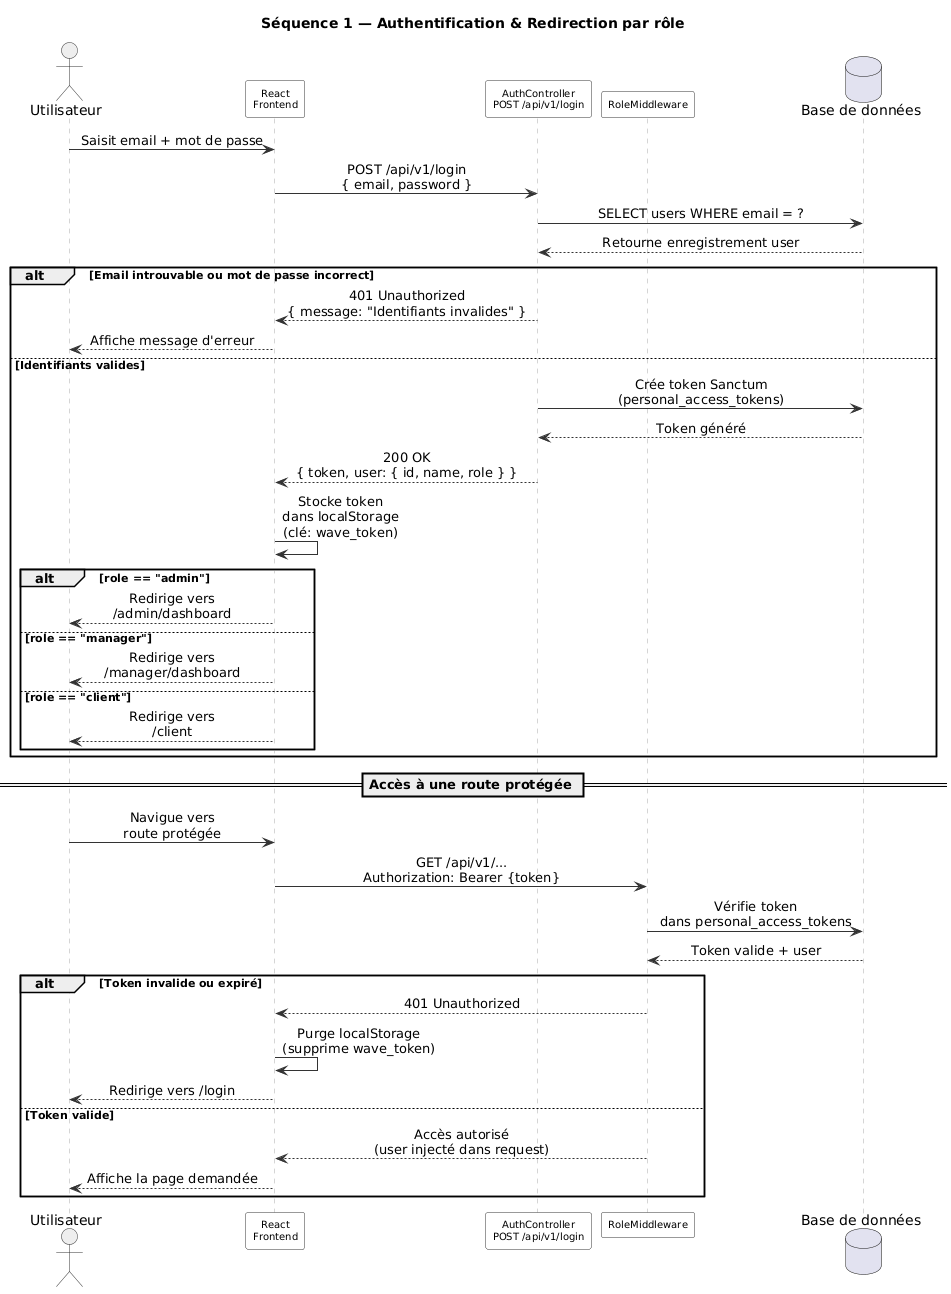
\includegraphics[width=\textwidth]{diagrammes-Sequances/authentification.png}
  \caption{Diagramme de sequence -- Authentification et redirection par role}
  \label{fig:seq1}
\end{figure}

\subsection{Sequence 2 -- Commande et paiement PayPal}

Le deuxieme diagramme de sequence (Figure \ref{fig:seq2}) retrace le
flux complet d'une commande depuis la boutique client jusqu'a l'attribution
automatique de la licence apres paiement confirme.

Le client parcourt le catalogue en appellant \texttt{GET /api/v1/client/shop},
qui retourne les produits dont le champ \texttt{is\_active} est vrai.
Quand il clique sur "Commander", le frontend envoie une requete POST vers
\texttt{/api/v1/client/shop/orders} avec l'identifiant du produit. Le
backend verifie que le produit est actif, recupere son prix, puis cree
un ordre PayPal via le SDK \texttt{srmklive/paypal} avec le montant en
MAD. L'identifiant et l'URL d'approbation PayPal sont retournes. Une
commande est inseree en base avec le statut \texttt{pending} et
l'identifiant PayPal. Le frontend redirige le client vers la page de
paiement PayPal via l'URL d'approbation.

Apres validation du paiement sur PayPal, le client est redirige vers
l'application. Le frontend envoie une requete POST vers
\texttt{/api/v1/client/shop/orders/\{order\_id\}/capture}. Le backend
recupere la commande, appelle \texttt{captureOrder} sur le SDK PayPal
avec l'identifiant PayPal. Si le paiement est refuse, le statut de la
commande est mis a \texttt{cancelled} et une erreur 402 est retournee.
Si la capture est confirmee, le backend met le statut a
\texttt{completed}, cree un enregistrement de paiement avec type
\texttt{license}, puis insere une entree dans la table pivot
\texttt{client\_license} avec les dates d'attribution et d'expiration
calculees automatiquement selon la duree du produit. Une reponse 200
confirme la commande et le frontend affiche les details de la licence
nouvellement activee.

\begin{figure}[H]
  \centering
  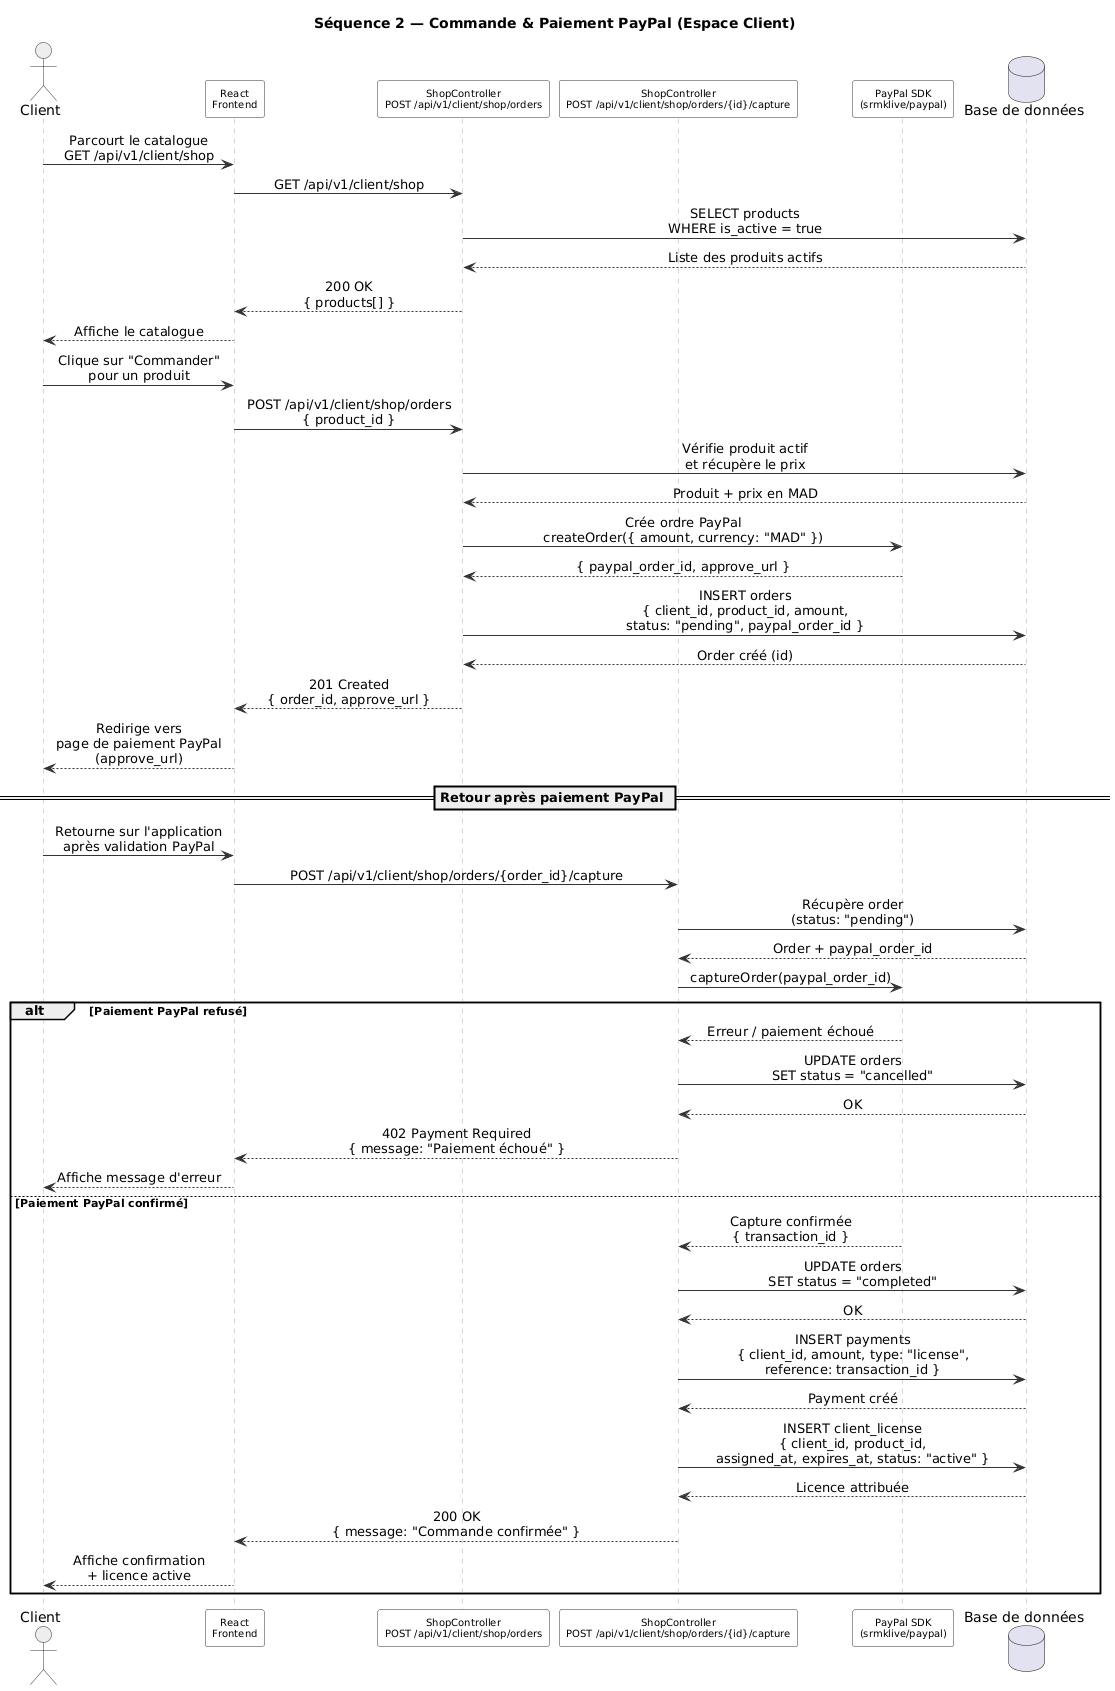
\includegraphics[width=\textwidth]{diagrammes-Sequances/paiment.png}
  \caption{Diagramme de sequence -- Commande et paiement PayPal}
  \label{fig:seq2}
\end{figure}

\subsection{Sequence 3 -- Verification automatique des licences}

Le troisieme diagramme de sequence (Figure \ref{fig:seq3}) illustre le
fonctionnement du systeme d'automatisation base sur le planificateur
de taches Laravel. Ce scenario ne fait intervenir aucune action manuelle
de la part d'un utilisateur : tout est declenche automatiquement.

Chaque jour a 08h00, le Scheduler dispatch le job \texttt{CheckLicenseExpiry}.
Ce job interroge la base pour recuperer toutes les licences dont la date
d'expiration est inferieure ou egale a la date du jour. Pour chacune d'elles,
il met a jour le statut a \texttt{expired}. Il effectue ensuite une seconde
requete pour identifier les licences dont l'expiration se situe entre
maintenant et dans sept jours. Pour chacune, il met le statut a
\texttt{expiring\_soon} et dispatch la notification
\texttt{LicenseExpiringNotification}. Cette notification est envoyee via
deux canaux en parallele : le canal \texttt{database}, qui insere une entree
dans la table \texttt{notifications} consultable depuis l'espace client,
et le canal \texttt{mail}, qui envoie un email via Laravel Mailer avec un
lien vers la boutique pour renouveler la licence.

Toujours a 08h00, le Scheduler dispatch le job
\texttt{SendLicenseExpiryReminder}. Celui-ci interroge la base pour trouver
les licences dont la date d'expiration correspond exactement a aujourd'hui
plus sept jours et dont le statut est \texttt{expiring\_soon}. Pour chaque
client concerne, il envoie individuellement un email de rappel avec un
lien vers la boutique.

Enfin, quand le client consulte ses notifications via
\texttt{GET /api/v1/client/notifications}, il recoit la liste des
notifications lues et non lues. Il peut ensuite marquer une notification
comme lue via \texttt{PATCH /api/v1/client/notifications/\{id\}/read},
ce qui retourne un 200 confirmant la mise a jour.

\begin{figure}[H]
  \centering
  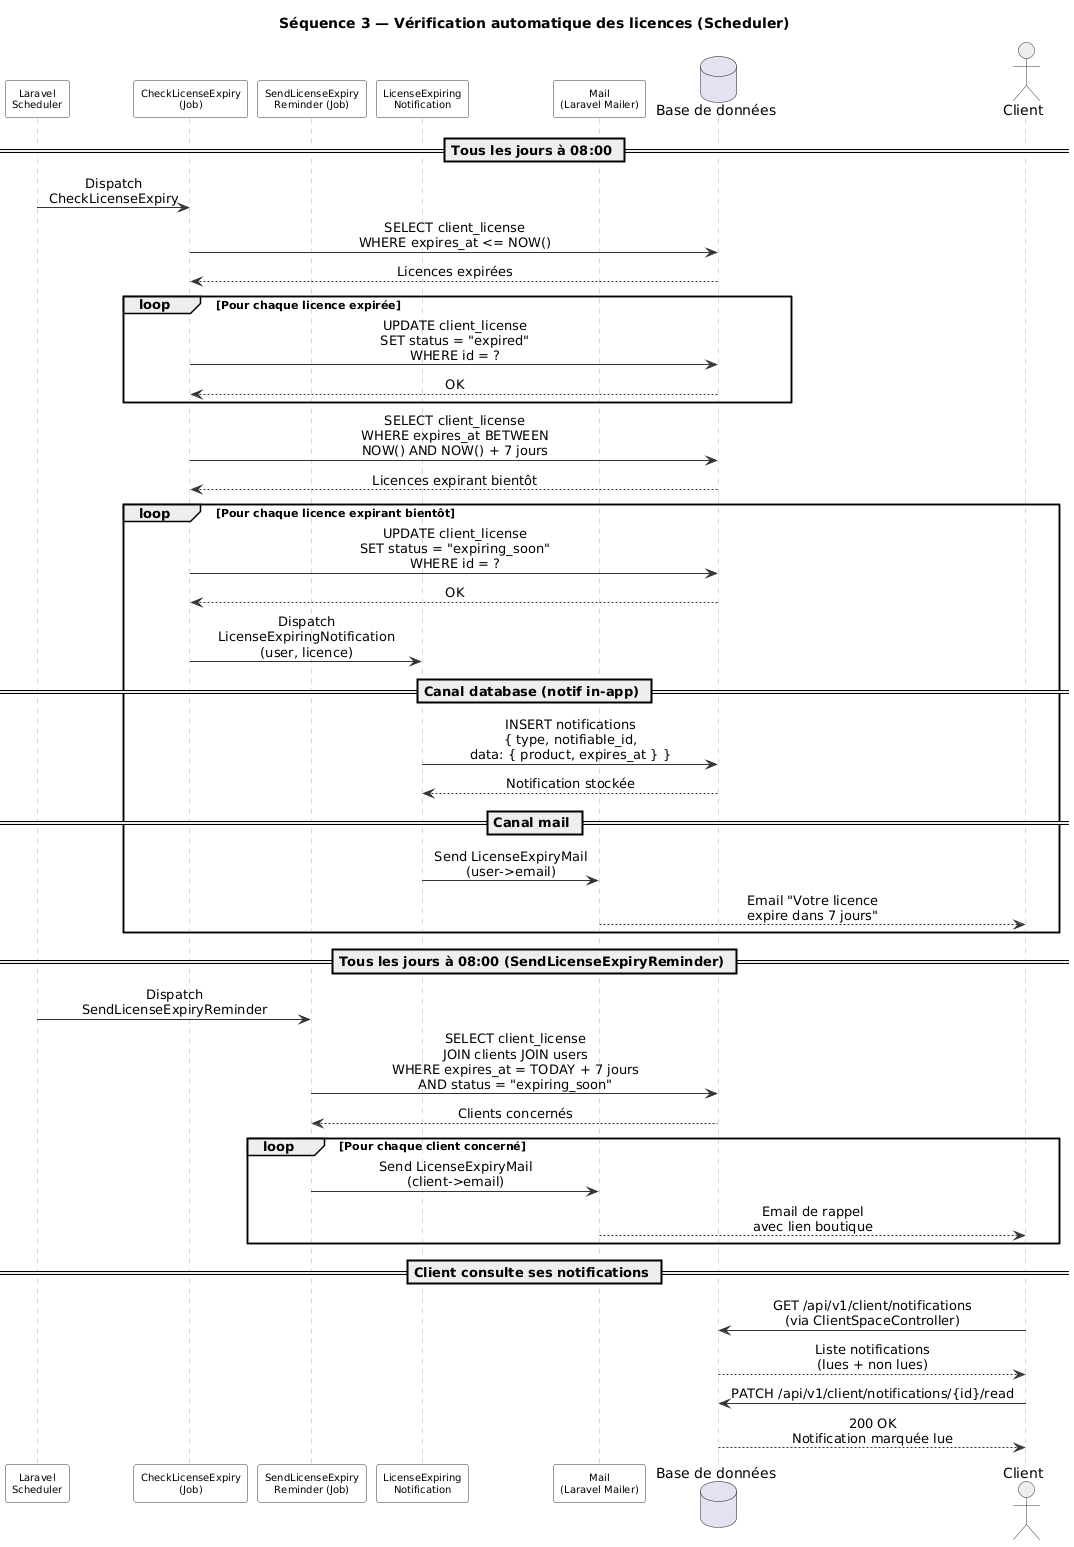
\includegraphics[width=\textwidth]{diagrammes-Sequances/verif-automatique des licences.png}
  \caption{Diagramme de sequence -- Verification automatique des licences}
  \label{fig:seq3}
\end{figure}

% ============================================================
\section{Diagramme de classes}
% ============================================================

Le diagramme de classes (Figure \ref{fig:classes}) represente la structure
statique du systeme. Il decrit les entites du domaine, leurs attributs,
leurs methodes et les relations qui les unissent. Il constitue la reference
directe pour la conception du schema de base de donnees.

\begin{figure}[H]
  \centering
  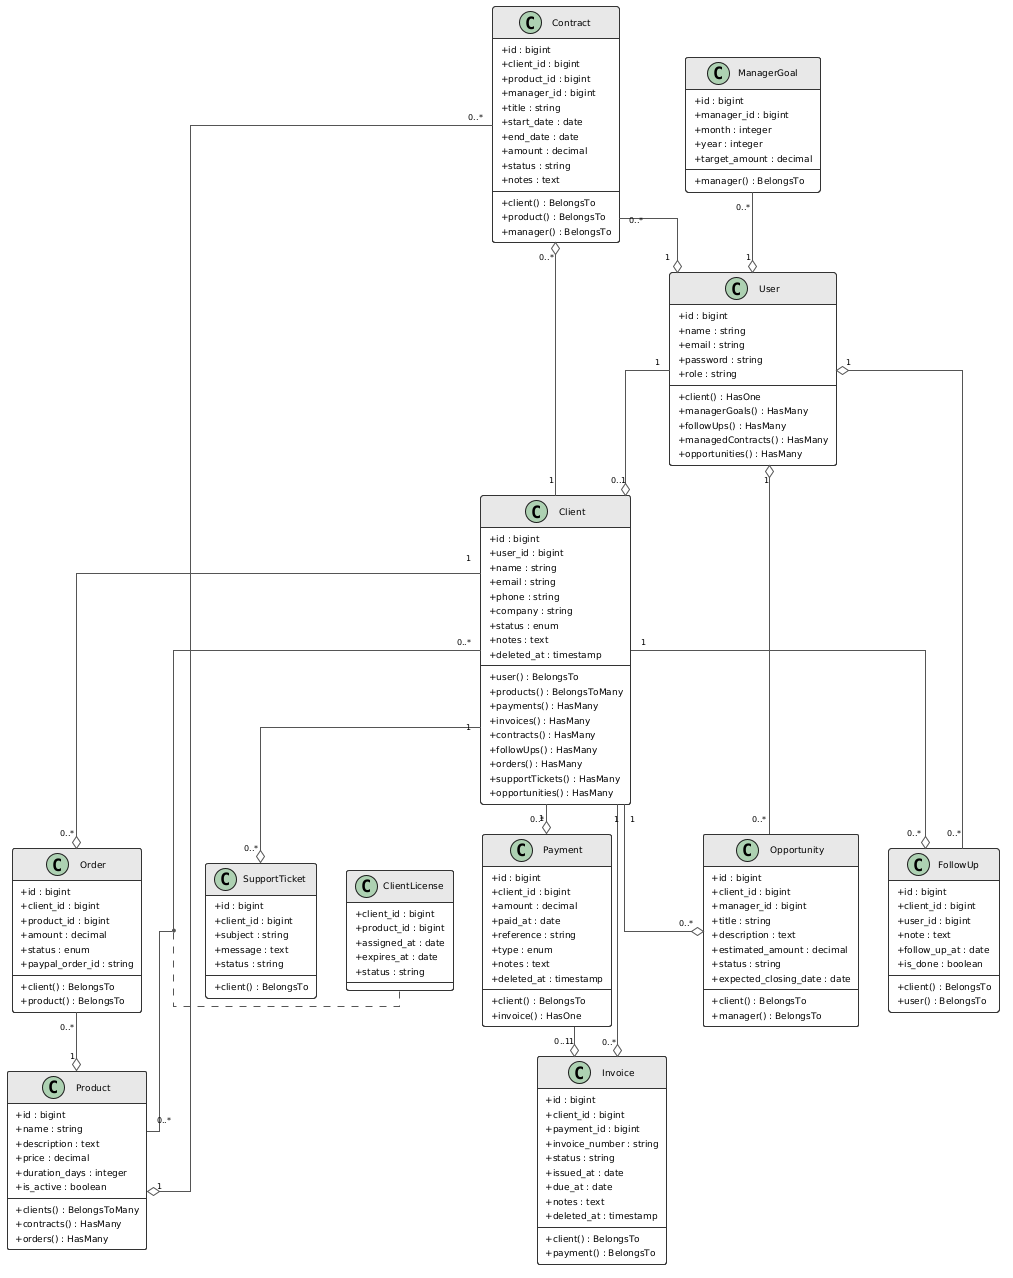
\includegraphics[width=\textwidth]{diagrammes-Classes/diag_classes.png}
  \caption{Diagramme de classes de l'application WAVE}
  \label{fig:classes}
\end{figure}

Le diagramme s'organise autour de deux entites centrales : \textbf{User}
et \textbf{Client}.

La classe \textbf{User} represente tout utilisateur authentifie dans le
systeme, quel que soit son role. Elle stocke les informations d'identite
(nom, email, mot de passe hache) et le champ \texttt{role} qui determine
les droits d'acces. Un User peut avoir une relation HasOne vers un Client
(dans le cas d'un utilisateur client provisionne par le manager), et des
relations HasMany vers les entites ManagerGoal, FollowUp, Contract
(en tant que manager responsable) et Opportunity.

La classe \textbf{Client} est la pierre angulaire de la logique metier.
Elle contient les informations commerciales du client (nom, email, telephone,
societe, statut, notes) et le champ \texttt{deleted\_at} qui permet les
suppressions douces. Un Client est relie a un User via une cle etrangere
\texttt{user\_id} nullable (nullable car un client peut exister sans
compte utilisateur). Il entretient des relations HasMany avec les classes
Payment, Invoice, Contract, FollowUp, Order et SupportTicket. La relation
avec Product est de type ManyToMany via la table pivot
\texttt{client\_license}, qui stocke les dates d'attribution et
d'expiration ainsi que le statut de chaque licence.

La classe \textbf{Product} stocke les informations du catalogue : nom,
description, prix en MAD, duree en jours et le flag \texttt{is\_active}
qui controle la visibilite en boutique. Elle est reliee a Client via la
table pivot \texttt{client\_license}, et a Contract et Order par des
relations BelongsTo.

La classe \textbf{Payment} enregistre chaque transaction financiere avec
son montant, sa date, sa reference et son type via un enum
(\texttt{subscription}, \texttt{license}, \texttt{other}). Elle supporte
les suppressions douces. Elle a une relation HasOne vers Invoice, ce qui
lie automatiquement une facture a son paiement d'origine.

La classe \textbf{Invoice} stocke les factures avec leur numero au format
\texttt{FAC-YYYY-NNNN}, leur statut, leurs dates d'emission et d'echeance.
Elle supporte les suppressions douces et est reliee a Client et Payment
via des cles etrangeres.

La classe \textbf{Contract} modelise les engagements contractuels entre
l'agence et ses clients. Elle reference a la fois le client, le produit
concerne et le manager responsable. Un scope Eloquent
\texttt{expiringWithin} est defini pour filtrer facilement les contrats
expirant dans un delai donne.

Les classes \textbf{Opportunity} et \textbf{FollowUp} couvrent
respectivement le pipeline commercial CRM et les relances commerciales.
Toutes deux referencent un client et un utilisateur manager. FollowUp
dispose d'un champ booleen \texttt{is\_done} pour marquer une relance
comme effectuee.

La classe \textbf{Order} enregistre les commandes passees via PayPal,
avec le champ \texttt{paypal\_order\_id} permettant de faire le lien
avec la transaction PayPal et un enum de statut
(\texttt{pending}, \texttt{completed}, \texttt{cancelled}).

La classe \textbf{SupportTicket} modelise les tickets de support soumis
par les clients, avec leur sujet, leur message et leur statut.

Enfin, la classe \textbf{ManagerGoal} stocke les objectifs mensuels
definis par l'admin pour chaque manager, avec le mois, l'annee et le
montant cible en MAD.

Le tableau \ref{tab:relations} synthetise les principales relations entre
les classes du systeme.

\vspace{0.4cm}
\begin{table}[H]
\centering
\caption{Principales relations Eloquent du systeme}
\label{tab:relations}
\begin{tabularx}{\textwidth}{@{}llX@{}}
\toprule
\textbf{Classe source} & \textbf{Type} & \textbf{Classe cible} \\
\midrule
User          & HasOne      & Client \\[3pt]
User          & HasMany     & ManagerGoal, FollowUp, Contract (manager), Opportunity \\[3pt]
Client        & BelongsTo   & User \\[3pt]
Client        & HasMany     & Payment, Invoice, Contract, FollowUp, Order, SupportTicket \\[3pt]
Client        & BelongsToMany & Product (via client\_license) \\[3pt]
Payment       & HasOne      & Invoice \\[3pt]
Invoice       & BelongsTo   & Client, Payment \\[3pt]
Contract      & BelongsTo   & Client, Product, User (manager) \\[3pt]
Opportunity   & BelongsTo   & Client, User (manager) \\[3pt]
Order         & BelongsTo   & Client, Product \\[3pt]
SupportTicket & BelongsTo   & Client \\[3pt]
ManagerGoal   & BelongsTo   & User (manager) \\
\bottomrule
\end{tabularx}
\end{table}

% ============================================================
\section{Architecture technique}
% ============================================================

\subsection{Architecture API-first}

L'application repose sur une architecture API-first avec une separation
nette entre le backend et le frontend. Le backend est un serveur Laravel
qui expose une API REST sous le prefixe \texttt{/api/v1}. Le frontend
est une Single Page Application React qui consomme cette API via des
requetes HTTP authentifiees. Les deux serveurs fonctionnent de maniere
independante et communiquent exclusivement par echanges JSON.

Cette separation offre plusieurs avantages concrets : le frontend peut
etre deploye sur un hebergeur statique sans dependre de l'infrastructure
PHP, le backend peut etre consomme par d'autres clients (application
mobile, outil tiers) sans modification, et les deux couches peuvent
evoluer independamment l'une de l'autre.

\subsection{Gestion des roles et des acces}

Le controle d'acces est implemente a deux niveaux. Cote backend, le
middleware \texttt{RoleMiddleware} verifie le champ \texttt{role} de
l'utilisateur authentifie avant d'autoriser l'acces a chaque groupe
de routes. Les routes admin sont protegees par
\texttt{middleware(['auth:sanctum', 'role:admin'])},  les routes
back-office par \\ \texttt{role:admin,manager}, 
et les routes espace
client par \texttt{role:client}.

Cote frontend, le composant \texttt{PrivateRoute} inspecte le role
stocke dans le contexte d'authentification et redirige automatiquement
tout utilisateur qui tenterait d'acceder a une section qui ne lui
appartient pas.

\subsection{Gestion asynchrone et taches planifiees}

Les operations longues ou susceptibles d'echouer, notamment l'envoi
d'emails, sont traitees de maniere asynchrone via le systeme de queues
de Laravel. Cela garantit que les actions de l'utilisateur recoivent
une reponse immediate sans attendre la fin de traitements externes.

Les taches recurrentes sont definies dans \texttt{routes/console.php}
et orchestrees par le scheduler Laravel, qui agit comme un cron unifie.
Les trois taches planifiees sont la verification quotidienne des licences
a 08h00, l'envoi des rappels de retard de paiement chaque lundi a 09h00
et la generation du rapport mensuel le premier de chaque mois a 07h00.

% ============================================================
\section{Conclusion}
% ============================================================

Ce deuxieme chapitre a pose les fondations conceptuelles et architecturales
de l'application WAVE. Les diagrammes de cas d'utilisation ont permis de
couvrir exhaustivement l'ensemble des interactions entre les quatre acteurs
du systeme et la plateforme. Les diagrammes de sequence ont mis en lumiere
les flux les plus complexes : la securisation de l'authentification par
token Bearer avec redirection par role, le processus de commande et de
paiement PayPal avec attribution automatique de licence, et le systeme
d'automatisation par taches planifiees pour le suivi des licences.

Le diagramme de classes a revele une architecture de donnees coherente,
organisee autour des entites Client et User, avec des relations Eloquent
bien definies qui facilitent les requetes et garantissent l'integrite
referentielle des donnees.

Ces elements constituent la reference directe qui a guide le developpement
technique. Le chapitre suivant presentera la realisation de l'application :
les choix technologiques justifies, les modules implementes et les
interfaces produites.